\documentclass[xcolor=table,xcdraw,aspectratio=169]{beamer}
\usepackage{beamerthemesplit}
\usepackage{wrapfig}
\usetheme{SPbGU}
\usepackage{pdfpages}
\usepackage{amsmath}
\usepackage{cmap} 
\usepackage[T2A]{fontenc} 
\usepackage[utf8]{inputenc}
\usepackage[english,russian]{babel}
\usepackage{indentfirst}
\usepackage{amsmath}
\usepackage{multirow}
\usepackage[noend]{algpseudocode}
\usepackage{algorithm}
\usepackage{algorithmicx}
\usepackage{csvsimple}
\usepackage{booktabs}
\usepackage{adjustbox}
% \usetikzlibrary{shapes,arrows}
\usepackage{fancyvrb}
\usepackage{algpseudocode}
\usepackage{algorithm}
\usepackage{algorithmicx}
\usepackage{verbatim}
\usepackage{mathtools}
\usepackage{multirow}
\usepackage{subcaption}

\usepackage{fontawesome}
\usepackage{array}

\usepackage{tikz}
\usetikzlibrary{automata,positioning}
\usepackage{svg}
% \usepackage[table,xcdraw]{xcolor}

\usepackage[most]{tcolorbox}

\newtheorem{rutheorem}{Теорема}
\newtheorem{ruproof}{Доказательство}
\newtheorem{rudefinition}{Определение}
\newtheorem{rulemma}{Лемма}
\beamertemplatenavigationsymbolsempty

\title[Модернизация CFPQ\_Data]{Модернизация набора данных \textsc{CFPQ\_Data}}
% То, что в квадратных скобках, отображается в левом нижнем углу. 
\institute[СПбГУ]{
Санкт-Петербургский государственный университет \\
Кафедра системного программирования }

% То, что в квадратных скобках, отображается в левом нижнем углу.
\author[Вадим Абзалов]{Вадим Игоревич Абзалов, 18.Б11-мм \\
  % У научного руководителя должна быть указана научная степень
  \and  
    {\bfseries Научный руководитель:} к.\,ф.-м.\,н., доцент кафедры информатики СПбГУ С.\,В. Григорьев}

\date{\today}

\definecolor{orange}{RGB}{179,36,31}

\begin{document}
{
% Лого университета или организации, отображается в шапке титульного листа
\begin{frame}
  \begin{center}
  {\includegraphics[width=1.5cm]{img/SPbGU_Logo.png}}
  \end{center}
  \titlepage
\end{frame}
}

\section{Introduction}

Scalable high-performance graph analysis is an actual challenge.
There is a big number of ways to attack this challenge~\cite{Coimbra2021} and the first promising idea is to utilize general-purpose graphic processing units (GPGPU).
Such existing solutions, as CuSha~\cite{10.1145/2600212.2600227} and Gunrock~\cite{7967137} show that utilization of GPUs can improve the performance of graph analysis, moreover it is shown that solutions may be scaled to multi-GPU systems.
But low flexibility and high complexity of API are problems of these solutions.

The second promising thing which provides a user-friendly API for high-performance graph analysis algorithms creation is a GraphBLAS API~\cite{7761646} which provides linear algebra based building blocks to create graph analysis algorithms.
The idea of GraphBLAS is based on a well-known fact that linear algebra operations can be efficiently implemented on parallel hardware.
Along with that, a graph can be natively represented using matrices: adjacency matrix, incidence matrix, etc.
While reference CPU-based implementation of GraphBLAS, SuiteSparse:GraphBLAS~\cite{10.1145/3322125}, demonstrates good performance in real-world tasks, GPU-based implementation is challenging.

One of the challenges in this way is that real data are often sparse, thus underlying matrices and vectors are also sparse, and, as a result, classical dense data structures and respective algorithms are inefficient. 
So, it is necessary to use advanced data structures and procedures to implement sparse linear algebra, but the efficient implementation of them on GPU is hard due to the irregularity of workload and data access patterns.
Though such well-known libraries as cuSPARSE show that sparse linear algebra operations can be efficiently implemented for GPGPU, it is not so trivial to implement GraphBLAS on GPGPU. 
First of all, it requires \textit{generic} sparse linear algebra, thus it is impossible just to reuse existing libraries which are almost all specified for operations over floats.
The second problem is specific optimizations, such as masking fusion, which can not be natively implemented on top of existing kernels.
Nevertheless, there is a number of implementations of GraphBLAS on GPGPU, such as GraphBLAST~\cite{yang2019graphblast}, GBTL~\cite{7529957}, which show that GPGPUs utilization can improve the performance of GraphBLAS-based graph analysis solutions.
But these solutions are not portable because they are based on Nvidia Cuda stack.
Moreover, the scalability problem is not solved: all these solutions support only single-GPU, not multi-GPU computations.

To provide portable GPU implementation of GraphBLAS API we developed a \textit{SPLA} library\footnote{Source code available at: \url{https://github.com/JetBrains-Research/spla}}.
This library utilizes OpenCL for GPGPU computing to be portable across devices of different vendors.
Moreover, it is initially designed to utilize multiple GPGPUs to be scalable.
To sum up, the contribution of this work is the following.
\begin{itemize}
    \item Design of portable GPU GraphBLAS implementation proposed. The design involves the utilization of multiple GPUS. Additionally, the proposed design is aimed to simplify library tuning and wrappers for different high-level platforms and languages creation. 
    \item Subset of GraphBLAS API, including such operations as masking, matrix-matrix multiplication, matrix-matrix e-wise addition, is implemented. The current implementation is limited by COO and CSR matrix representation format and uses basic algorithms for some operations, but work in progress and more data formats will be supported and advanced algorithms will be implemented in the future.
    \item Preliminary evaluation on such algorithms as breadth-first search (BFS) and triangles counting (TC), and real-world graphs shows portability across different vendors and promising performance: for some problems Spla is comparable with GraphBLAST. Surprisingly, for some problems, the proposed solution on embedded Intel graphic card shows better performance than SuiteSparse:GraphBLAS on the respective CPU. At the same time, the evaluation shows that further optimization is required.
\end{itemize} 
\begin{frame}[fragile]
	\transwipe[direction=90]
	\frametitle{\faGithub\ Проект \textsc{CFPQ\_Data}}
	
	\begin{columns}
        \begin{column}{0.5\textwidth}
            \textbf{Экспериментальное исследование CFPQ алгоритмов}
            \begin{enumerate}
                \item[\bullet] Проводить на реальных данных
                \item[\bullet] Определять производительность
                \item[\bullet] Cравнить с уже существующими решениями
                \item[\textcolor{red}{\faWarning}] \textbf{\textcolor{red}{Нет единого набора данных}}
            \end{enumerate}
        \end{column}

        \begin{column}{0.5\textwidth}
            \textbf{Проект \textsc{CFPQ\_Data}}
            \begin{itemize} 
        	    \item[\textbf{(1/2)}] Множество различных реальных и синтетических графов
                \item[\textbf{(2/2)}] Вспомогательные инструменты
                \item[\textcolor{red}{\faWarning}] \textbf{\textcolor{red}{Имеет ряд технических ограничений}}
            \end{itemize}
        \end{column}
    \end{columns}
\end{frame}

\begin{frame}[fragile]
	\transwipe[direction=90]
	\frametitle{\faLegal\ Требования к проекту \textsc{CFPQ\_Data}}
	
	\begin{columns}
        \begin{column}{0.5\textwidth}
            \textbf{Проблемы}
            \begin{itemize}
                \item[\textcolor{red}{\faQuestion}] Набор данных может быть загружен только целиком
                \item[\textcolor{red}{\faQuestion}] Отсутствуют инструменты манипулирования графами
                \item[\textcolor{red}{\faQuestion}] Отсутствует информация о структуре графов, включенных в набор
            \end{itemize}
        \end{column}

        \begin{column}{0.5\textwidth}
            \textbf{Требования}
            \begin{itemize} 
        	    \item[\textcolor{green}{\faCheck}] Предоставить возможность загрузки конкретного графа из набора
                \item[\textcolor{green}{\faCheck}] Предоставить инструменты для манипулирования графами
                \item[\textcolor{green}{\faCheck}] Предоставить информацию о структуре графов, включенных в набор
            \end{itemize}
        \end{column}
    \end{columns}
\end{frame}

% Обязательный слайд: четкая формулировка цели данной работы и постановка задачи
% Описание выносимых на защиту результатов, процесса или особенностей их достижения и т.д.
\begin{frame}
	\transwipe[direction=90]
	\frametitle{\faThumbTack\ Цель и задачи}
	\textbf{Цель}: модернизация существующего набора данных \textsc{CFPQ\_Data} для создания унифицированного средства подготовки проведения экспериментального исследования CFPQ алгоритмов
	  
	~\
	  
	\textbf{Задачи}
	
	\newline
	
	\begin{itemize}
		\item[\bullet] Модернизация архитектуры набора данных
		\item[\bullet] Добавление новых возможностей работы с данными
		      \begin{itemize}
		      	\item[\bullet] Загрузка конкретных графов из набора данных
		      	\item[\bullet] Преобразование графов в другие форматы
		      	\item[\bullet] Получение информации о графе
		      	\item[\bullet] Трансформация графов
		      \end{itemize}
% 		\item[\bullet] Разработка и реализация протокола версионирования данных
		\item[\bullet] Публикация Python пакета для работы с набором данных и документации к нему
	\end{itemize}
	
\end{frame}


\section{Обзор}

Для того чтобы упростить ход рассуждений, касающихся контекстно-свободных грамматик, в данной работе используется понятие \textit{рекурсивного автомата} --- абстракции, позволяющей задавать произвольную КС-грамматику.
Ее описание приводится в первом параграфе обзора. 
Второй параграф посвящен вопросу о разрешимости задачи синтаксического анализа контекстно-свободного представления данных и его связи с фундаментальными проблемами теории формальных языков.

Предлагаемый в данной работе алгоритм основан на алгоритме синтаксического анализа регулярных множеств, который, в свою очередь, явлется модификацией алгоритма обобщенного синтаксического анализа Generalized LL. 
Об этих алгоритмах, а также о проекте, в рамках которого проведена разработка предложенного решения, также будет рассказано в обзоре.

\subsection{Рекурсивные автоматы и КС-грамматики}
Введем понятие рекурсивного автомата, которое потребуется для дальнейшего изложения

\begin{defn}
	Рекурсивный автомат R --- это пятерка $(\Sigma, Q, \delta, q_0, q_f)$, где $\Sigma$ --- конечное множество терминальных символов, $Q$ --- конечное множество состояний автомата, $\delta : Q \times (\Sigma \cup Q) \rightarrow 2^Q$ --- функция переходов, $q_0 \in Q$ --- начальное состояние, $q_f$ --- конечное состояние. 
\end{defn}

Можно заметить, что данное определение практически идентично определению стандартного конечного автомата. 
Единственное отличие состоит в том, что метками на ребрах рекурсивного автомата могут как терминальные символы (терминальные переходы), так и состояния (нетерминальные переходы).
Класс рекурсивных автоматов обладает такой же выразительностью, как и контекстно-свободные грамматики, т.е. позволяет описать любой контекстно-свободный язык. 
Более того, грамматика тривиальным образом может быть преобразована в рекурсивный автомат (обратное тоже верно) \cite{tellier2006ra}. 
Пример рекурсивного автомата, построенного по грамматике, можно увидеть на рисунке \ref{fig:ra_ex}.

\begin{figure}[h]
	\centering
	\begin{subfigure}[b]{0.45\textwidth}
		\centering
		$$
		\begin{array}{crcl}
		&S' & ::= & S \\
		&S  & ::= & \texttt{[ } S \texttt{ ]}\\
		&S  & ::= & \mbox{\texttt{a}}
		\end{array}
		$$
		\caption{Грамматика $G_1$}
	\end{subfigure}
	~
	\begin{subfigure}[b]{0.45\textwidth}
		\centering
		\includegraphics[width=4cm]{pictures/ra_example.pdf}
		\caption{Рекурсивный автомат для $G_1$}
	\end{subfigure}
	\caption{Преобразование между грамматикой и рекурсивным автоматом}
	\label{fig:ra_ex}
\end{figure}


\subsection{Разрешимость задачи синтаксического анализа контекстно-свободного представления}
Как было сказано ранее, задачу поиска шаблона, при условии, что и шаблон, и данные, в которых осуществляется поиск, представлены контекстно-свободными грамматиками, мы назовем синтаксическим анализом контекстно-свободного представления. 

Для доказательства предложений, сформулированных далее, будет использоваться следующая теорема \cite{Nederhof}.

\begin{theorem}[Nederhof, Satta]
	Пусть $G_1$ --- произвольная контекстно-свободная грамматика, $G_2$ --- грамматика, которая не содержит непосредственной или скрытой рекурсий. Тогда проблема проверки пустоты пересечения языков, порождаемых данными грамматиками, относится к классу PSPACE-complete.
\end{theorem}

Рассмотрим случай, когда грамматика данных задает ровно одну строку. Пусть $G_t$ --- произвольная КС-грамматика, задающая шаблоны для поиска, а $G_d$ --- КС-грамматика, которая не содержит непосредственной или скрытой рекурсий. $L(G_t)$ и $L(G_d)$ --- языки, порождаемые грамматиками, при этом $L(G_d) = \{\omega\}$, где $\omega$ --- исходные данные, к которым был применен алгоритм сжатия. 
Необходимо определить, существуют ли такие строки $\omega'$, что $\omega' \in L(G_t)$ и $\omega'$ --- подстрока $\omega$.

%т.е. $\omega' \in L_{sub}(\omega)$, где $L_{sub}(s)$ --- обозначение для языка, состоящего из всех подстрок заданной строки $s$. Отметим, что $L_{sub}$ относится к классу регулярных языков, так как множество всех подстрок конечно. 

\begin{prop}
	При выполнении описанных условий задача синтаксического анализа КС-представления разрешима.
\end{prop}

\begin{proof}
Пользуясь эквивалентностью представлений, можно записать грамматику $G_d$ в виде рекурсивного автомата $R_d$. Рассмотрим рекурсивный автомат $R_{i,\,j}$, полученный из $R_d$ путем замены стартового состояния на $i \in Q(R_d)$ и назначения терминирующего (финального, из которого не может быть совершено переходов) состояния $j \in Q(R_d)$. Такой автомат описывает грамматику, которая является представленим некоторой подстроки $\omega$. 
%В таком случае, рекурсивный автомат $R_{i,\,j}$, полученный из $R_d$ путем замены стартового и конечного состояний на $i, j \in Q(R_d)$ соответственно, описывает грамматику, которая является представленим некоторой подстроки $\omega$. 
Рассмотрев все возможные пары $i$ и $j$, получаем конечное множество грамматик, для каждой из которых необходимо проверить, содержится ли строка, порождаемая ей, в языке $L(G_t)$. 
Согласно теореме 1, такая проверка является разрешимой задачей и принадлежит к классу PSPACE-complete.
\end{proof}

Отдельно отметим, что для описанных процедур используется лишь исходный автомат, эквивалентный грамматике $G_d$. 
Условия задачи поиска шаблонов непосредственно в контекстно-свободном представлении, таким образом, выполняются. 
Верна также разрешимость более общей задачи.

\begin{prop}
	Пусть грамматика $G_d$ задает конечное множество строк $L(G_d) = \{\omega_1, \, \dots \, , \omega_n \}$. Необходимо определить, существуют ли строки $\omega'$, для которых верно: $\omega' \in L(G_t)$ и $\omega'$ --- подстрока одной из строк $\omega_i \in L(G_d)$. Данная задача разрешима и принадлежит классу PSPACE-complete.
\end{prop}

\begin{proof}
	Как и в предыдущем доказательстве, используем запись грамматики в виде рекурсивного автомата $R_d$ и рассмотрим автоматы $R_{i, j}$. В данном случае каждый из этих автоматов представляет собой грамматику, которая порождает некоторое конечное множество подстрок исходных строк из $L(G_d)$. Проверка пустоты пересечения такой грамматики с $G_t$ также соответствует условиям теоремы 1.
\end{proof}

В случае, когда грамматика $G_d$ представляет собой бесконечный регулярный язык (т.е. содержит левую и/или правую рекурсию), разрешимость задачи поиска шаблонов установить не удается. Подход, использованный ранее в доказательстве предложений, не может быть применен, так как части рекурсивного автомата, представляющего грамматику $G_d$, также могут содержать рекурсивные переходы, что выходит за рамки условия теоремы 1. Проверка разрешимости и определение класса сложности задачи проверки пустоты пересечения произвольной и регулярной КС-грамматик в настоящее время остаются открытыми проблемами \cite{Nederhof}.

%Пусть $G$ --- произвольная КС-грамматика, $M$ --- конечный автомат. Тогда задача проверки
%\begin{itemize}
%	\item включения языков ($L(M) \subseteq L(G)$) --- неразрешима
%	\item пустоты пересечения ($L(M) \cap L(G) = \emptyset$) --- разрешима (т.к. в пересечении не более чем КС-язык) за полиномиальное время \cite{Hunt}
%	\item регулярности языка $L(G)$ --- неразрешима \cite{Greibach1968}
%\end{itemize} 
%
%Если использовать представление регулярного языка $L(M)$ в виде КС-грамматики $G_r$, то задача проверки пустоты пересечения ($L(G_r) \, \cap \, L(G) = \emptyset$) становится немного интереснее: если $G_r$ 
%\begin{itemize}
%	\item нерекурсивная --- задача из PSPACE \cite{Nederhof} (точнее результата нет (я не нашел, по крайней мере))
%	\item лево- или праволинейная --- ничего не известно (см. последний абзац заключения из \cite{Nederhof})
%	\item принадлежит еще более широкому классу --- тем более ничего не известно
%\end{itemize}

%Еще немного про вложенную рекурсию и регулярность языка. Грамматика без вложенной рекурсии (NSE) порождает регулярный язык \cite{Chomsky} (обратное тоже верно, для регулярного языка можно построить NSE грамматику, т.к. праволинейная, например, --- частный случай NSE). Существует алгоритм, который позволяет проверять грамматику на наличие вложенной рекурсии за полином \cite{Anselmo}. Однако, грамматика с вложенной рекурсией тоже может порождать регулярный язык \cite{Andrei2004}, поэтому задача о проверке регулярности языка, порождаемого КС-грамматикой, остается неразрешимой. 

\subsection{GLL-алгоритм и его модификации}

Классические алгоритмы нисходящего и восходящего синтаксического анализа предполагают использование грамматики, которая является в достаточной мере однозначной. 
В противном случае, управляющие таблицы анализаторов содержат конфликты, из-за чего нельзя гарантировать корректное поведение на любых входных данных. 
Для работы с сильно неоднозначными грамматикам используются алгоритмы \textit{обобщенного синтаксического анализа}, которые позволяют рассмотреть все возможные пути разбора строки и построить соответствующие деревья вывода.
Поиск шаблонов не требует наличия деревьев вывода, поэтому в дальнейшем алгоритмы синтаксического анализа рассматриваются только как механизм, позволяющий определить принадлежность строки языку.

\subsubsection{Оригинальный GLL-алгоритм}

Generalized LL (GLL) \cite{gll} --- алгоритм, обобщающий идеи нисходящего синтаксического анализа. GLL, в отличие от стандартных LL-алгоритмов, позволяет использовать для анализа произвольную \linebreak контекстно-свободную грамматику, в том числе содержащую леворекурсивные правила. Вместе с тем, GLL наследует такие полезные свойства алгоритмов нисходящего анализа, как непосредственная связь с грамматикой и простота отладки и диагностики ошибок.

Для обработки неоднозначностей GLL разделяет стек анализатора на несколько ветвей, каждая из которых соответствует возможному пути разбора. При таком подходе необходимо компактное представление множества стеков, в качестве которого выступает Graph Structured Stack (GSS). В работе \cite{Afroozeh2015gss} была представлена модификация GSS, которая позволяет увеличить эффективность GLL-анализа. Вершины такого представления хранят в себе номер нетерминала и позицию в строке, с которой начался разбор подстроки, соответствующей ему. На ребрах хранятся позиции в грамматике (вида $X \rightarrow \alpha A \cdot \beta$), на которые необходимо вернуться после завершения разбора нетерминала. 
%При помощи GSS также решается проблема бесконечного роста стеков при обработке левой рекурсии: при попытке создать вершину, которая уже существует, в граф добавится

Основной идеей GLL является использование дескрипторов, позволяющих полностью описывать состояние анализатора в текущий момент времени.

\begin{defn}
	Дескриптор --- это тройка (L, u, i), где
	\begin{itemize}
		\setlength\itemsep{0em}
		\item L --- текущая позиция в грамматике вида $A \rightarrow \alpha \cdot \beta$
		\item u --- текущая вершина GSS
		\item i --- позиция во входном потоке 
	\end{itemize}
\end{defn}  

В процессе работы поддерживается глобальная очередь дескрипторов. В начале каждого шага исполнения алгоритм берет следующий в очереди дескриптор и производит действия в зависимости от позиции в грамматике и текущего входного символа, передвигая соответствующие указатели. 
При наличии конфликтов в грамматике алгоритм добавляет дескрипторы для каждого возможного пути анализа в конец очереди.

\subsubsection{Поддержка грамматик в EBNF}

В работе Артема Горохова \cite{Gorokhov2017ebnf} была описана модификация GLL, которая позволяет использовать грамматики, записанные в расширенной форме Бэкуса-Наура (EBNF). Грамматика такого вида трансформируется в соответствующий рекурсивный автомат, в котором затем минимизируется количество состояний. Синтаксический анализ производится без построения управляющих таблиц: алгоритм обходит рекурсивный автомат в соответствии со входным потоком символов. При обработке текущего дескриптора $(C_S, C_U, i)$, где $C_S$ --- вершина автомата (эквивалент позиции в грамматике), $C_U$ --- вершина GSS, $i$ --- позиция в строке, могут возникать следующие ситуации.

\begin{itemize}
	\item $C_S$ --- финальное состояние. Показывает, что разбор текущего нетерминала был завершен. Необходимо осуществить возврат из $C_U$ по меткам на исходящих из нее ребрах.
	\item Присутствует нетерминальный переход из $C_S$. В данном случае необходимо начать разбор указанного нетерминала $X$. Для этого в GSS должна быть создана новая вершина $(X, i)$, если она не создавалась ранее, а текущая вершина автомата изменена на стартовую для $X$.
	\item Присутствует терминальный переход из $C_S$. Необходимо сравнить терминал на ребре автомата с текущим входным символом. Если они совпадают, то осуществить переход в вершину автомата, на которую указывает ребро, и передвинуть указатель в строке.
\end{itemize}

За счет уменьшения количества состояния в автомате удается достичь прироста в производительности по сравнению со стандартным GLL-алгоритмом. 

\subsubsection{Синтаксический анализ графов}

Стандартными входными данными для алгоритмов синтаксического анализа являются линейные последовательности токенов. На основе GLL был разработан алгоритм, который позволяет производить синтаксический анализ регулярных множеств строк, представленных в виде конечного автомата (который, в свою очередь, является ориентированным графом с токенами на ребрах).

Поддержка нелинейного входа не потребовала существенных изменений в оригинальном алгоритме. Дескрипторы модифицированного алгоритма хранят номер вершины входного графа вместо позиции в строке. Также, на шаге исполнения просматривается не единственный текущий символ, а множество символов на ребрах, исходящих из текущей вершины.

Производительность данного алгоритма, как и обычного GLL, может быть увеличена при помощи представления входной грамматики в виде рекурсивного автомата. В таком случае, алгоритм будет производить обход двух автоматов --- рекурсивного и конечного. Ситуации, возникающие при обработке дексрипторов, не отличаются от описанных ранее ситуаций для линейного входа. Псевдокод данной модификации приведен в приложении.

\subsection{Проект YaccConstructor}

YaccConstructor --- исследовательский проект лаборатории языковых инструментов JetBrains на математико-механическом факультете СПбГУ, направленный на исследования в области лексического и синтаксического анализа. Проект включает в себя одноименную модульную платформу для разработки лексических и синтаксических анализаторов, содержащую большое количество компонент: язык описания грамматик YARD, преобразования над грамматиками и др. Основным языком разработки является F$\#$.

Ранее в рамках YaccConstructor были реализованы генераторы GLL-анализаторов, описание которых было приведено в данном обзоре. 

\chapter{Инструментальный пакет} \label{relWorks}

В данной главе описан инструментальный пакет (Software Development Kit, SDK) \textbf{YC.SEL.SDK}, предназначенный для разработки различных решений по статическому анализу динамически формируемых выражений. Представлена архитектура разработанного SDK, а также архитектура надстройки \textbf{YC.SEL.SDK.ReSharper}, позволяющей создавать расширения для ReSharper, предоставляющие поддержку встроенных языков. Изложенный выше алгоритм синтаксического анализа реализован в рамках одной из компонент SDK. YC.SEL.SDK и YC.SEL.SDK.ReSharper являются \textbf{платформами} для разработки инструментов статического анализа динамически формируемого кода.

\section{Архитектура}

Практически любой язык программирования может использоваться как встроенный. Даже если рассматривать только SQL, то окажется, что у него множество различных диалектов, каждый из которых имеет свои особенности. Внешним языком также может быть любой язык программирования. Трудность заключается в том, что  любое из сочетаний внешнего и встроенного языка может встретиться на практике, и задачи, которые необходимо решать в этой ситуации, могут быть различными (поиск ошибок, подсчёт метрик, автоматизация трансформаций и т.д.). Реализовать универсальный инструмент, решающий все задачи для всех языков, не представляется возможным. Более целесообразно создать набор инструментов, упрощающий создание конечных решений для конкретных языков и конкретных задач. В качестве примера можно рассмотреть инструменты для разработки компиляторов, которые включают в себя генераторы лексических, синтаксических анализаторов и набор библиотек с вспомогательными функциями, и тем самым упрощают создание конкретного компилятора для выбранного языка и целевой платформы.

Требуемый набор инструментов для работы со встроенными языками должен поддерживать весь процесс обработки кода, который может выглядеть так, как представлено на рисунке~\ref{fig:SeqSelProcessing}. Можно выделить следующие основные шаги.
\begin{itemize}
    \item Анализ основного кода, который выполняется сторонним инструментом. Результат этого шага --- это дерево разбора с информацией, достаточной для выполнения дальнейших шагов.
    \item Построение аппроксимации множества возможных значений динамически формируемых выражений.
    \item Лексический анализ построенной на предыдущем шаге аппроксимации.
    \item Синтаксический анализ, результатом которого является лес разбора, пригодный для дальнейшей обработки.
    \item Обработка леса разбора, вычисление семантики.
\end{itemize}

На каждом шаге может быть получена информация, полезная для пользователя, такая как список ошибок, и её необходимо отобразить для него соответствующим образом.

\begin{figure}[h!]
\begin{center}
\includegraphics[width=0.9\textwidth]{pics/Activ_SEL_Processing}
\caption{Диаграмма последовательности обработки встроенных языков}
\label{fig:SeqSelProcessing} 
\end{center}
\end{figure}


Существующие инструменты для работы со встроенными языками обычно реализуют поддержку какого-то фиксированного набора языков. При этом поддержка нового языка, как правило, требует нетривиальнй доработки инструмента. Чтобы получить поддержку встроенного языка без изменений в исходном коде базового инструмента, необходимо предоставить соответствующий механизм. 

Для того чтобы упростить процесс создания конечных инструментов, создан SDK, одной из компонент которого является генератор синтаксических анализаторов на основе предложенного в данной работе алгоритма. Также в него входит генератор лексических анализаторов, библиотека построения регулярной аппроксимации, набор вспомогательных функций. Подробное описание компонент приведено далее.

Так как анализ внешнего языка является сложной самостоятельной задачей, то он не включён в разработанный SDK. На вход созданному на основе SDK инструменту должно подаваться дерево разбора внешнего языка с информацией, достаточной для решения поставленных в данной работе задач. 


\subsection{Архитектура YS.SEL.SDK}

Разработанный SDK включает компоненты, необходимые для реализации шагов, представленных на рисунке ~\ref{fig:SeqSelProcessing} и описанных ранее, за исключением анализа внешнего языка. Архитектура SDK изображена на рисунке~\ref{fig:SDKHLArch} и включает в себя генераторы анализаторов и различные библиотеки времени исполнения.

\begin{figure}[h!]
\begin{center}
\includegraphics[width=0.9\textwidth]{pics/HighLevelArch}
\caption{Архитектура SDK целиком}
\label{fig:SDKHLArch} 
\end{center}
\end{figure}

Так как анализ внешнего языка не входит в задачи разработанного SDK, то первый шаг, выполнение которого необходимо обеспечить, --- это построение аппроксимации. В нашем случае строится регулярное приближение множества значений динамически формируемого выражения.

Построение регулярной аппроксимации основано на алгоритме, изложенном в работе~\cite{RegOverApprox}, который позволяет строить приближение сверху для множества значений выражений. То есть $L_R$, задаваемый регулярным приближением, не меньше, чем $L_1$, задаваемый программой (выполняется включение $L_R \in L_1$). Это позволяет говорить о надёжности дальнейших анализов в том смысле, что они не теряют информации о $L_1$. Например, это важно при поиске ошибок. Если в $L_R$ не обнаружено ошибок (то есть $L_R \in L_2$, где $L_2$ --- эталонный), значит и в $L_1$ ошибок нет. При этом могут быть найдены ошибки в $L_R$, которых нет в $L_1$, то есть будут ложные срабатывания. Однако наличие ложных срабатываний лучше, чем пропущенные ошибки, и их количество может быть уменьшено путём повышения точности аппроксимации. 

Для того чтобы сделать построение приближения независимым от внешнего языка, реализовано обобщённое представление графа потока управления (Control Flow Graph, CFG)~\cite{Dragon}, которое содержит всю необходимую для дальнейшей работы информацию. Таким образом, разработчику необходимо реализовать построение обобщённого представления CFG для конкретного внешнего языка. В результате компонента строит конечный автомат, являющийся приближением множества значений динамически формируемых выражений.

Компонента, отвечающая за лексический анализ, состоит из двух частей: генератора лексических анализаторов, который по описанию лексики обрабатываемого языка строит соответствующий конечный преобразователь, и интерпретатора, который производит анализ входной структуры данных на основе построенного генератором преобразователя. Архитектура компоненты представлена на рисунке~\ref{fig:LexArch}. На вход принимается конечный автомат над символами, результатом работы является конечный автомат над алфавитом токенов анализируемого языка. Входной конечный автомат может быть построен с помощью компоненты построения регулярной аппроксимации. Основные структуры данных --- конечный автомат и конечный преобразователь --- и функции работы с ними описаны в соответствующей библиотеке.

\begin{figure}[h!]
\begin{center}
\includegraphics[width=0.95\textwidth]{pics/LexerDiagram}
\caption{Архитектура лексического анализатора}
\label{fig:LexArch} 
\end{center}
\end{figure}

Лексический анализатор реализован на основе инструмента FsLex, который является стандартным генератором лексических анализаторов для языка F\#. При реализации был переиспользован язык описания лексики и некоторые структуры данных.

Реализованный генератор лексических анализаторов обладает следующими особенностями.
\begin{itemize}
    \item Поддерживаются разрывные токены, то есть токены формируемые из нескольких строковых литералов.
    \item Сохраняется привязка лексических единиц к исходному коду: сохраняется информация о строковом литерале, из которого породился токен и координаты его внутри этой строки. Так как одна лексическая единица может формироваться из нескольких строковых литералов, то привязка сохраняется отдельно для каждой части.
    \item Поддерживается обработка входных конечных автоматов, содержащих циклы.
    \item Так как значение токена может формироваться с помощью цикла и, как следствие, быть бесконечным, то каждый токен содержит конечный автомат, порождающий все возможные значения для данного токена, а не единственное значение, как это реализовано в классическом лексическом анализе.
\end{itemize}

\textbf{Генератор синтаксических анализаторов}, названный ARNGLR, реализован на основе алгоритма, описанного в разделе~\ref{AlgoDescr}. Его архитектура представлена на рисунке~\ref{fig:ParsArch}.  

\begin{figure}[h!]
\begin{center}
\includegraphics[width=0.95\textwidth]{pics/ARNGLRArch}
\caption{Архитектура синтаксического анализатора}
\label{fig:ParsArch} 
\end{center}
\end{figure}

Генератор реализован как один из модулей YC и может принимать на вход внутреннее представление грамматики (IL), которое может быть получено с помощью различных фронтендов (Frontends), однако в рамках YC.SEL.SDK 
основным фронтендом является YARD, так как он предоставляет наиболее развитые средства для описания грамматик. По грамматике обрабатываемого языка строятся управляющие таблицы анализатора, которые сохраняются в файле Parser.fs. 
Построенные таблицы должны быть включены в разрабатываемое приложение UserApplication. Интерпретатор, предназначенный для синтаксического разбора конечного автомата, полученный после лексического анализа, реализован 
в виде отдельной библиотеки ARNGLR.Runtime, которая также должна быть подключена к разрабатываемому приложению. В результате работы интерпретатора будет получен SPPF, который может быть использован для дальнейшей 
обработки (например, подсчёта метрик). Для упрощения работы с SPPF реализован ряд вспомогательных функций.

\subsection{Архитектура YC.SEL.SDK.ReSharper}

ReSharper --- это расширение к Microsoft Visual Studio IDE, предоставляющее широкий спектр  дополнительной функциональности по анализу и рефакторингу кода. ReSharper поддерживает несколько языков, например C\#, Visual Basic .NET, JavaScript, и этот список может быть расширен благодаря наличию свободно распространяемого ReSharper SDK, описание которого было представлено ранее в разделе~\ref{ReSharperSDKDescr}. ReSharper.SDK позволяет получить деревья разбора для поддерживаемых языков, предоставляет набор готовых анализов и упрощает взаимодействие с Microsoft Visual Studio IDE и её компонентами. Более того, предоставляется возможность разработки собственных расширений для ReSharper на основе ReSharper.SDK.

Microsoft Visual Studio является достаточно распространённой средой разработки, но не поддерживает встроенные языки, поэтому было решено разработать ряд расширений к ReSharper с использованием разработанного инструментария, которые будут устранять данный недостаток. Стоит отметить, что не ставилось задачи поддержать все встроенные языки, так как встроенным может быть любой язык программирования. Также не было необходимости поддержать все внешние языки программирования. Необходимо на базе разработанного YC.SEL.SDK создать инфраструктуру, позволяющую реализовывать поддержку новых встроенных языков в Microsoft Visual Studio через расширения к ReSharper и реализовать несколько расширений, демонстрирующих возможности созданной инфраструктуры. 

Так как необходимо поддерживать различные языки, то необходимо обеспечить расширяемость по новыми языками. Классический подход к решению такой задачи для интегрированных сред разработки заключается в том, что поддержка нового языка реализуется в виде независимой компоненты. Если пользователь хочет получить поддержку какого-либо языка в своей среде разработки, то он должен установить соответствующий пакет. При этом поддержка различных языков осуществляется независимо, однако часто выделяется общая функциональность, которая может быть оформлена в виде отдельного пакета.

Для предоставления описанных выше возможностей была реализована надстройка над YC.SEL.SDK, упрощающая создание расширений для ReSharper, названная  YC.SEL.SDK.ReSharper. В неё включены компоненты, реализующие функции, которые упрощающают взаимодействие YC.SEL.SDK и ReSharper.SDK. Назначени основных из них описаны ниже.

\begin{itemize}
  \item Общая точка расширения, необходимая для подключения функциональности для различных встроенных языков, которая может быть реализована в различных расширениях, к ReSharper через общий интерфейс. Также общая точка расширения позволяет использовать общую функциональность, необходимую для работы со встроенными языками.
  \item Отображение в IDE информации, полученной в ходе анализа. Например, подсветка синтаксиса и ошибок. Вывод диагностических сообщений с информацией об ошибках.
  \item Преобразование данных, из формата, используемого в ReSharper.SDK, в формат для YC.SEL.SDK. Например, преобразование графа потока управления внешнего языка, построенного ReSharper.SDK, в формат, пригодный для построения регулярной аппроксимации средствами YC.SEL.SDK.
  \item Управление работой анализаторов, необходимое, с одной стороны, для обеспечения своевременной реакции на изменения в коде, совершённые пользователем, а с другой, для прекращения вычислений, результаты которых уже не актуальны. Управление построено на основе общего для ReSharper механизма, обеспечивающего асинхронную работу анализов. При этом вычисления могут быть прерваны, если, например, пользователь внёс в код изменения, делающие анализ или его результаты некорректными. 
\end{itemize}

Как уже говорилось, встроенными могут быть различные языки и учесть заранее все их особенности не представляется возможным. Кроме того, даже при использовании одного встроенного языка могут использоваться различные способы выполнения сформированного запроса. Таким образом, необходимо предоставлять возможность настройки расширений конечным пользователем. Для этого в рамках YC.SEL.SDK.ReSharper была реализована возможность управления следующими основными параметрами расширений. 

\begin{itemize}
    \item Подсветка синтаксиса для каждого языка. Предоставлена возможность указать цвет для каждого типа токена.
    \item Указание парных элементов. Для каждого языка можно указать, какие лексические единицы считать парными: для каждой пары указывается ``левый'' (открывающая скобка) и ``правый'' (закрывающая скобка) элементы. При расположении курсора в тексте рядом с одним из элементов пары будут подсвечены соответствующие элементы. Пример подсветки парных элементов приведён на рисунке~\ref{fig:braces}.
    \item Точки интереса или хотспоты (hotspot) --- это места, в которых должно быть сформировано финальное выражение. Необходимо знать, какой хотспот какому языку соответствует. При этом нужно учитывать, что одному языку может соответствовать несколько хотспотов. Например, динамически сформированный SQL-запрос в программе на языке программирования C\# может быть выполнен с помощью метода \verb|ExecuteQuery| класса \verb|DataContext|~\cite{ExecuteQuery}
     или же текст запроса может быть передан как аргумент конструктора класса \verb|SqlCommand|~\cite{SqlCommand} с последующим выполнением с помощью метода \verb|ExecuteReader|.

\end{itemize}

Настройка указанных выше параметров хранится в соответствующих конфигурационных файлах в формате XML, которые на данный момент редактируются вручную. Настройка подсветки синтаксиса и парных элементов совмещена в одном файле и для каждого языка создаётся отдельный такой файл. Конфигурационный файл с точками интереса является общим для всех языков и, соответственно, для всех установленных расширений для поддержки встроенных языков.

В листинге~\ref{lst:codeHighlighting} приведён пример конфигурации подсветки синтаксиса и парных скобок для языка Calc. Для указания цвета используются имена, принятые в ReSharper (например, \verb|"CONSTANT_IDENTIFIER_ATTRIBUTE"|), что должно сделать настройку цветов более единообразной. В xml-тэге \verb|Matched| содержится описание парных элементов. Каждая пара описывается в xml-тэге \verb|Pair| и для одного языка может быть указано более одной такой пары.

\fvset{frame=lines,framesep=5pt}
\begin{listing}[H]
    \begin{pyglist}[language=xml,numbers=left,numbersep=5pt]
<?xml version="1.0" encoding="utf-8"?>
<SyntaxDefinition name="CalcHighlighting">
    <Colors>
        <Tokens color="CONSTANT_IDENTIFIER_ATTRIBUTE">
            <Token> DIV </Token>
            <Token> LBRACE </Token>
            <Token> MINUS </Token>
            <Token> MULT </Token>
            <Token> NUMBER </Token>
            <Token> PLUS </Token>
            <Token> POW </Token>
            <Token> RBRACE </Token>
        </Tokens>
    </Colors>
<!-- Dynamic highlighting: -->
    <Matched>
        <Pair>
            <Left> LBRACE </Left>
            <Right> RBRACE </Right>
        </Pair>
<!-- You can specify more then one pair:        
        <Pair>
            <Left> LEFT_SQUARE_BRACKET </Left>
            <Right> RIGHT_SQUARE_BRACKET </Right>
        </Pair>
        <Pair>
            <Left> LEFT_FIGURE_BRACKET </Left>
            <Right> LEFT_FIGURE_BRACKET </Right>
        </Pair>
-->        
    </Matched>
</SyntaxDefinition>
    \end{pyglist}
\caption{Пример конфигурационного файла для настройки подсветки синтаксиса}
\label{lst:codeHighlighting}
\end{listing}

Листинг~\ref{lst:hotspots} содержит пример описания точек интереса. Для каждой точки интереса должна быть указана следующая информация.
\begin{itemize}
    \item Какому встроенному языку соответствует точка. Информация хранится в Xml-тэге \verb|Language|.
    \item Полное имя метода, являющегося точкой интереса. Информация хранится в Xml-тэге \verb|Method|.
    \item Порядковый номер аргумента данного метода, являющегося выражением на встроенном языке. Нумерация начинается с нуля. Информация хранится в Xml-тэге \verb|ArgumentPosition|. 
    \item Возвращаемый тип метода.  Информация хранится в Xml-тэге \verb|ReturnType|. 
\end{itemize}

\fvset{frame=lines,framesep=5pt}
\begin{listing}[H]
    \begin{pyglist}[language=xml,numbers=left,numbersep=5pt]
<?xml version="1.0" encoding="utf-8"?>
<!-- comment about body -->
<Body>
    <!-- comment about hotspot -->
  <Hotspot>
      <!-- comment about tsql -->
      <Language> TSQL </Language>
      <!-- comment about fullName -->
      <Method>Program.ExecuteImmediate</Method>
      <!-- zero-based -->
      <ArgumentPosition> 0 </ArgumentPosition>
      <!-- comment about return type -->
      <ReturnType> void </ReturnType>
  </Hotspot>
  <Hotspot>
      <Language> Calc </Language>
      <Method>Program.Eval</Method>
      <ArgumentPosition> 0 </ArgumentPosition>
      <ReturnType> int </ReturnType>
  </Hotspot>
</Body>
    \end{pyglist}
\caption{Пример конфигурационного файла для настройки точек интереса}
\label{lst:hotspots}
\end{listing}


\section{Области и способы применения YC.SEL.SDK}

Разработанный SDK предназначен для создания инструментов статического анализа динамически формируемых строковых выражений. Решения, созданные с его помощью, могут применяться для работы с проектами, активно использующими динамически формируемые строковые выражения. Необходимость работать с такими проектами может возникнуть, например, в следующих областях.

\begin{itemize}
    \item Реинжиниринг программного обеспечения.
    \item Поддержка встроенных языков в средах разработки.
    \item Оценка качества и сложности кода.
\end{itemize}

Общим для всех этих областей является то, что для решения многих задач необходимо структурное представление динамически формируемого кода. При этом анализируемые языки могут быть различными и процесс их анализа часто тесно связан с анализом внешнего языка.

Отметим, что встроенные языки используются всё менее активно в молодых проектах и системах. На смену им приходят более надёжные способы композиции языков и метапрограммирования. Например LINQ или ORM-технологии. Однако это не всегда так. Использование строковых выражений для взаимодействия с базами данных и генерации WEB-страниц в приложениях на PHP всё ещё широко распространено~\cite{DSQLInActiveUse}. Это необходимо учитывать при поддержке встроенных языков в средах разработки. Для каких-то языков на первый план выходят возможности по изучению и модификации уже созданного кода, а для каких-то --- возможность быстро и удобно создавать новый код. Во втором случае могут возникнуть дополнительные требования к скорости работы инструмента, так как подразумевается выполнение некоторых операций ``на лету'', что может послужить ограничением на использование SDK, так как многие механизмы, реализованные в нём, не предусматривают возможности уменьшения точности в пользу увеличения быстродействия. Оценка качества и сложности  кода часто может выполняться в рамках комплекса задач по реинжинирингу системы, однако может быть и самостоятельной задачей, например, при оценке сложности работ по поддержке и сопровождению информационной системы.

Детали применения SDK могут варьироваться в зависимости от решаемых задач и контекста использования. Например, механизм построения регулярной аппроксимации может быть реализован независимо в рамках внешнего инструмента. Однако основной сценарий использования аналогичен использованию инструментариев для разработки компиляторов. Последовательность шагов, представленная ниже, может быть изменена в зависимости от особенностей задачи.

\textbf{Шаг 1.} Создание грамматики обрабатываемого языка. Грамматика может быть создана на основе документации соответствующего языка или переиспользована готовая, что оправданно, например, при создании анализатора для динамического SQL, когда внешний и встроенный языки совпадают.

\textbf{Шаг 2.} Генерация синтаксического анализатора по созданной грамматике. Для этого используется генератор синтаксических анализаторов, присутствующий в SDK. Результатом работы генератора является файл с исходным кодом на языке программирования F\#, который должен быть включён в разрабатываемый код. Файл содержит описание типов для лексических единиц, управляющие таблицы анализатора и функцию, которая по конечному автомату над алфавитом токенов анализируемого языка построит SPPF, содержащий деревья вывода всех корректных цепочек.

\textbf{Шаг 3.} Создание лексической спецификации обрабатываемого языка. Спецификация может быть извлечена из документации или заимствована из других проектов. При обработке динамически формируемого SQL возможно переиспользовать спецификацию, созданную для основного языка, которым также является SQL. При этом необходимо обратить внимание на то, что типы лексических единиц определяются на основе созданного на предыдущих шагах синтаксического анализатора.

\textbf{Шаг 4.} Генерация лексера по созданной спецификации. Для этого применяется генератор лексических анализаторов, входящий в состав SDK. В результате его применения получается файл с исходным кодом на языке F\#, который должен быть подключён к разрабатываемому решению. 

\textbf{Шаг 5.} Реализация механизма построения регулярной аппроксимации, результатом которого является функция, строящая конечный автомат над алфавитом символов. Данный механизм может быть реализован либо на основе предоставляемого в рамках SDK, либо независимо. В первом случае от разработчика требуется построить обобщённый CFG для внешнего языка. Во втором случае необходимо только гарантировать правильность возвращаемого конечного автомата. Второй подход может быть использован, например, при наличии реализованного механизма протягивания констант для внешнего языка. Это позволит создать возможно менее точное, но, скорее всего, более быстрое построение аппроксимации. Такой подход применим при автоматизированном реинжиниринге, когда ручная доработка кода является обязательным шагом и абсолютная точность автоматической обработки не требуется. Ещё одна возможная область применения второго подхода --- это поддержка встроенных языков в средах разработки. Здесь также часто не требуется высокая точность для подсказок пользователю, однако производительность крайне важна. Поэтому иногда приходится жертвовать точностью анализа для достижения нужной скорости работы.

\textbf{Шаг 6.} Реализация работы с SPPF. Синтаксический анализатор возвращает SPPF --- конечное представление леса разбора всех корректных цепочек из аппроксимации. Дальнейшая работа с ним может строиться по двум основным сценариям.

Превый сценарий --- непосредственная обработка SPPF. В этом случае все вычисления происходят над SPPF без извлечения отдельных деревьев. Это позволит ускорить обработку результатов разбора, так как количество деревьев может быть бесконечным, а SPPF является конечной структурой данных. Однако существует несколько проблем, связанных с таким подходом. Во-первых, требуется создание новых процедур обработки, так как классические, как правило, ориентированы на работу с деревьями. Во-вторых, могут возникнуть трудности при выполнении некоторых анализов, вызванные тем, что в SPPF хранятся ``бесконечные'' деревья. Например, необходимо вычислить максимальную глубину вложенности конструкции \verb|if|, являющуюся одной из стандартных метрик сложности кода. SPPF может содержать 
циклы и может оказаться так, что конструкция \verb|if| встречается в цикле таким образом, что потенциальная глубина вложенности может быть бесконечной. Такая ситуация не является стандартной при 
обработке деревьев разбора и её надо отслеживать отдельно.

Второй сценарий --- извлечение отдельных деревьев из SPPF и их обработка. Данный подход может оказаться удобным, если уже существуют процедуры обработки синтаксических деревьев для языка, который оказался встроенным. Это помогает избежать затрат на создание новой функциональности. Такое может произойти при работе с динамическим SQL. В этом случае для работы с деревом разбора внешнего языка и деревьями, извлечёнными из SPPF, можно использовать одни и те же процедуры, так как языки идентичны.

Недостатком второго подхода является то, что конечность числа деревьев не гарантирована. Это значит, что не удастся обработать все деревья. Стоит отметить, что даже в случае конечности числа деревьев, перебор и обработка всех деревьев разбора может потребовать значительных ресурсов.


\textbf{Шаг 7.} Реализация механизмов сбора, обработки и отображения информации, такой как сообщения об ошибках или любой другой, полученной в процессе анализа. Необходимо для предоставления пользователю информации, ожидаемой в рамках решаемой задачи.

На рисунке~\ref{fig:activMethod} изображён один из возможных сценариев использования SDK. Особенностью является цикличность процесса, характерная, например для реинжиниринга программного обеспечения.

\begin{figure}[h!]
\begin{center}
\includegraphics[width=0.9\textwidth]{pics/ActivMethodology}
\caption{Один из возможных вариантов использования SDK в проектах по реинжинирингу}
\label{fig:activMethod} 
\end{center}
\end{figure}

Встраивание анализа строковых выражений в последовательность обработки кода всей системы зависит от решаемых задач. Первыми шагами идут действия, необходимые для того, чтобы получить входные данные для анализа. Для этого необходимо провести лексический и синтаксический анализ внешнего языка, построить граф потока управления. После этого возможно построение аппроксимации и дальнейший анализ встроенных языков. Параллельно с этим может проводиться дальнейшая обработка внешнего языка. Степень параллельности зависит от независимости решаемых задач. Например, некоторые метрики сложности для основного кода и для динамически формируемого можно считать независимо и выводить отдельно. С другой стороны, может возникнуть необходимость вычислить некую комплексную метрику, учитывающую параметры и внешнего и динамически формируемого кода, что приведёт к необходимости синхронизации.

\section{Особенности реализации}

Разработка инструментального пакета с описанной выше архитектурой и плагинов для ReSharper велась в рамках исследовательского проекта YaccConstructor (YC), описанного в разделе~\ref{YCDescr}. 
Разработка велась на платформе .NET и основной язык реализации --- F\#~\cite{FSharp}. Весь исходный код опубликован на GitHub~\cite{YCUrl}. 
Большинство компонент опубликовано под ``открытой'' лицензией Apache License Version~2.0~\cite{ApacheV2}. 

За основу алгоритма синтаксического анализа динамически формируемых выражений был взят реализованный в YC алгоритм синтаксического анализа RNGLR. Генератор управляющих таблиц был использован практически без 
модификаций, а интерпретатор был реализован отдельный. Кроме этого, общими являются некоторые структуры данных и вспомогательные функции, такие как представление леса разбора и его печать в формате 
DOT~\footnote{DOT --- текстовый язык описания графов~\cite{DOT}.}, представление GSS. 

Лексичекий анализ реализован на основе инструмента FsLex, который потребовал значительных доработок для того, чтобы обеспечить обработку конечного автомата, а не линейного входа. Все остальные компоненты, 
необходимые для статического анализа динамически формируемых выражений, такие как построение аппроксимации, вспомогательные функции для упрощения построения целевых инструментов были реализованы ``с нуля'' 
в рамках проекта YC.

Бинарные пакеты, содержащие основную функциональность, опубликованы в сети интернет на NuGet~\footnote{NuGet --- менеджер пакетов для платформы .NET и одноимённый ресурс для их публикации. Позволяет публиковать 
и устанавливать пакеты, автоматически отслеживать зависимости между ними~\cite{NuGet}.}.

\begin{frame}[fragile]
	\transwipe[direction=90]
	\frametitle{\faCode\ Добавление новых возможностей}
	
	\begin{columns}
        \begin{column}{0.5\textwidth}
            \begin{figure}[t]{\textwidth}
				\centering
				\includegraphics[width=0.96\textwidth]{img/graphs.pdf}
				\caption*{Рис. 5. Модуль работы с графами} \label{fig:graphs}
			\end{figure}
        \end{column}

        \begin{column}{0.5\textwidth}
            \begin{figure}[t]{\textwidth}
				\centering
				\includegraphics[width=0.96\textwidth]{img/grammars.pdf}
				\caption*{Рис. 6. Модуль работы с грамматиками} \label{fig:grammars}
			\end{figure}
        \end{column}
    \end{columns}
\end{frame}

\begin{frame}[fragile]
	\transwipe[direction=90]
	\frametitle{\faCloudUpload\ Публикация пакета}
	
	\begin{columns}
        \begin{column}{0.75\textwidth}
            \begin{figure}[h]{\textwidth}
        		\centering
        		\tcbox[color=black,boxsep=0mm, boxrule=0.3mm,colback=white]{
        		    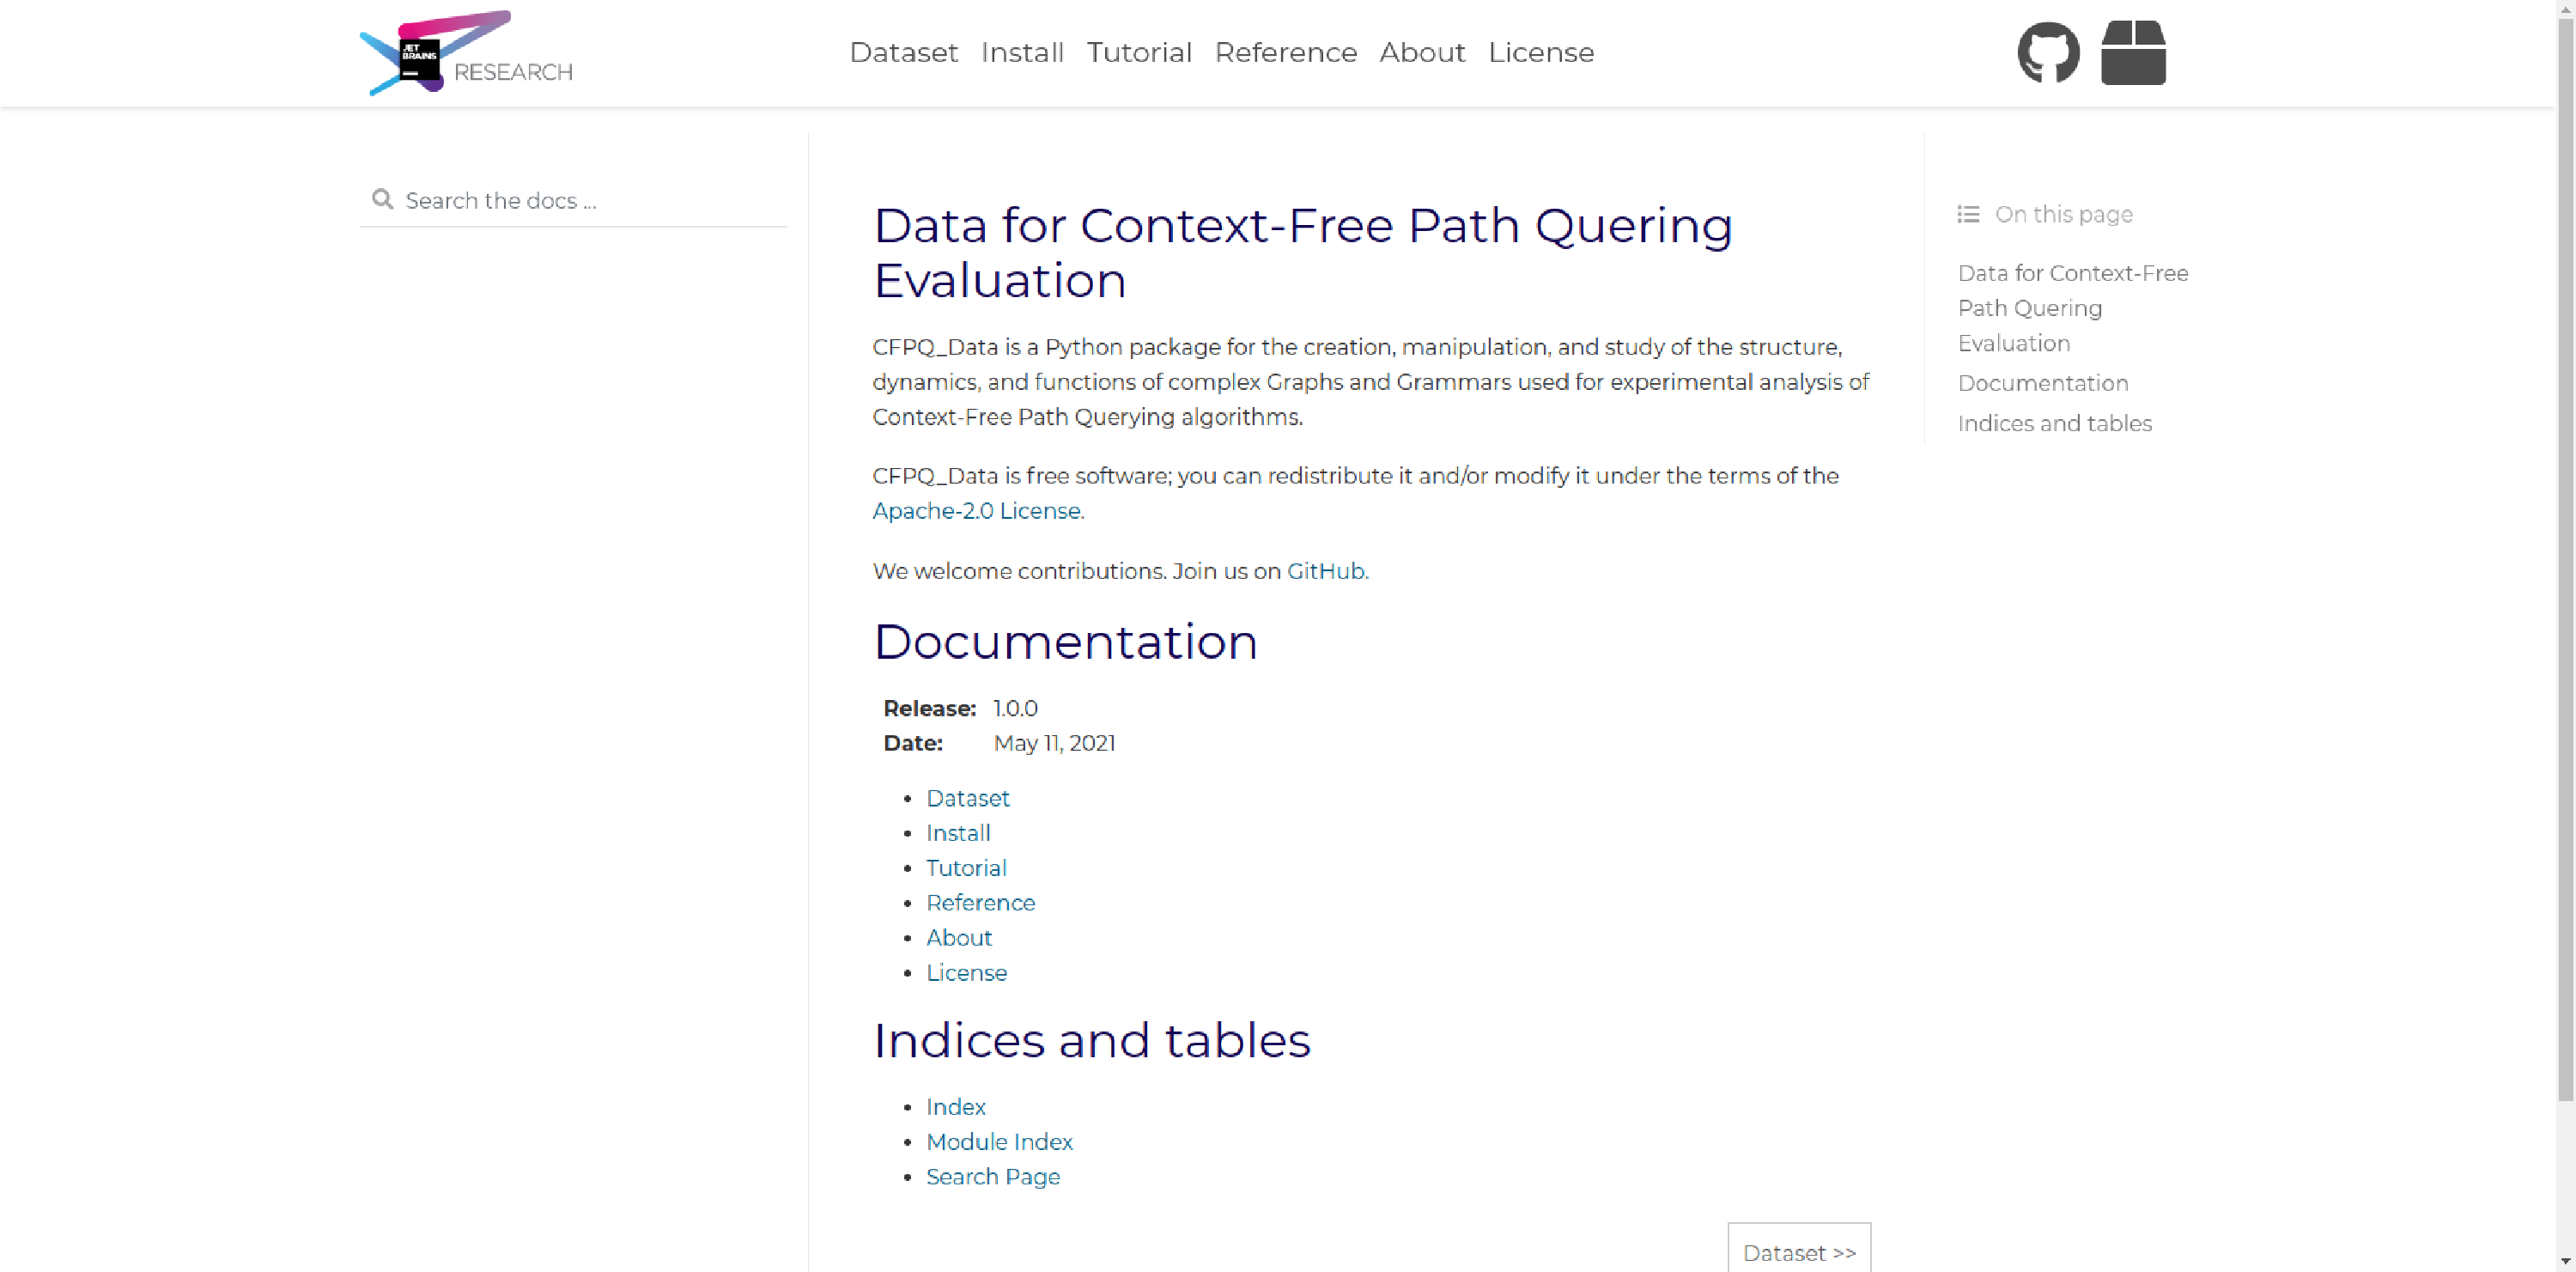
\includegraphics[height=0.6\textheight]{img/website_new.pdf}
        		}
        		\caption*{Рис. 8. Веб-сайт проекта} \label{fig:website}
        	\end{figure}
        \end{column}

        \begin{column}{0.25\textwidth}
            \begin{itemize} 
        	    \item[\bullet] Информация о наборе данных
        	    \item[\bullet] Руководство по установке
        	    \item[\bullet] Обучающее руководство
        	    \item[\bullet] Документация
            \end{itemize}
        \end{column}
    \end{columns}
\end{frame}

\section{\bf Modified Valiant's algorithm}

In this section we describe the reorganization of submatrices processing order in the Valiant's algorithm which simplify independent handling of submatrices. As a result, proposed modification can facilitate implementation of parallel submatrix processing.

\subsection{\bf \it Layered submatrices processing}

The main change of this modification is the possibility to divide the parsing table into layers of disjoint submatrices of the same size.
The idea of division we have made from the reorganization of the matrix multiplication order is presented in figure~\ref{fig2}.
Each layer consists of square matrices which size is power of 2.
The layers are computed successively in the bottom-up order.
Each matrix in the layer can be handled independently, which can help to implement parallel version of layer processing function.

\begin{figure}[h]
\vspace{3mm}
 \begin{center}
 \includegraphics[width=12cm]{pictures/modivis2.pdf}
    \caption{An example of the modification of Valiant's algorithm}
    \label{fig4}
 \end{center}
\vspace{-8mm}
\end{figure}

A simple example of the modification is shown in figure~\ref{fig4}.
The lowest layer (submatrices which size is 1) is already computed and filling of the matrix starts with the second layer (subfigures 1-2).
Note that the same process is presented in figure~\ref{fig3}, but here it can be done only in two steps using parallel computation of submatrix products.

The modified version of Valiant's algorithm is presented in listing~\ref{algo:modified}.
The procedure \textit{main()} computes the lowest layer $(T_{l, l+1})$, and then divide the table into layers, described earlier, and computes them through the \textit{completeVLayer()} call.
Thus, \textit{main()} computes all elements of parsing table $T$.
(Hereinafter, we use layer to mean set of submatrices.)

For brevity, we define \textit{left(subm), right(subm), top(subm), bottom(subm), \linebreak rightgrounded(subm)} and \textit{leftgrounded(subm)} functions which returns the submatrices for matrix $subm = (l, m, l', m')$ according to the original Valiant's algorithm (figure~\ref{fig2}).

Also denote some subsidiary functions for matrix layer $M$:
\begin{itemize}[noitemsep, nolistsep]
    \item[$-$] \textit{bottomsublayer(M)} $ = \{bottom(subm)\, |\,subm \in M \}$,
    \item[$-$] \textit{leftsublayer(M)} $ = \{\textit{left(subm)}\, |\,subm \in M \}$,
    \item[$-$] \textit{rightsublayer(M)} $ =\{\textit{right(subm)}\, |\,subm \in M \}$,
    \item[$-$] \textit{topsublayer(M)} $ = \{top(subm)\, |\,subm \in M \}$.
\end{itemize}

\begin{algorithm}[!h]
\SetAlgoNoLine
\KwIn{$G = (\Sigma, N, R, S), w = a_{1} \dots a_{n}, n \geq 1, n + 1 = 2^p, a_{i} \in \Sigma$ }
\underline{main()}{:}{

 \For {$l \in \{1, \ldots, n \}$}{$T_{l, l + 1} = \{A | A \rightarrow a_{l + 1} \in R\}$}
 \For{$1 \le i < p - 1 $}{
 layer = \textit{constructLayer(i)}\;
 \textit{completeVLayer(layer)}
 }
 accept if and only if $S \in T_{0, n}$
 \BlankLine
 }

\underline{constructLayer(i)}{:}{
 \BlankLine
 $\{(k2^i, (k+1)2^i, (k + 1)2^i, (k+2)2^i) \, |\, 0 \le k < 2^{p - i} - 1\}$
 \BlankLine
    }
\underline{completeLayer(M)}{:}{
\BlankLine
\If {$\forall (l, m, l', m') \in M \quad (m - l = 1)$}{\For{$ (l, m, l', m') \in M$}{$T_{l, l'} = f(P_{l, l'})$\;}}
\Else{
\textit{completeLayer(bottomsublayer(M))}\;
\textit{completeVLayer(M)}
}
\BlankLine
}

\underline{comleteVLayer(M)}{:}{
 \BlankLine
 \textit{multiplicationTasks$_1$ = \linebreak
    \{$left(subm)$, $leftgrounded(subm)$, $bottom(subm)\, |\,subm \in M \} \cup \linebreak  \{right(subm), bottom(subm), rightgrounded(subm)\, |\,subm \in M\}$\;}
 \BlankLine
 multiplicationTask$_2$ = $\{top(subm), leftgrounded(subm), right(subm)\, |\,subm \in M\}$\;
 \BlankLine
 multiplicationTask$_3$ = $\{top(subm), left(subm), rightgrounded\, |\,subm \in M\}$\;
 \BlankLine
 \textit{performMultiplications(multiplicationTask$_1$)}\;
 \textit{completeLayer(leftsublayer(M) $\cup$ rightsublayer(M))}\;
 \textit{performMultiplications(multiplicationTask$_2$)}\;
 \textit{performMultiplications(multiplicationTask$_3$)}\;
 \textit{completeLayer(topsublayer(M))}

 }
 \BlankLine

 \underline{performMultiplication(tasks)}{:}{\\
 \For{$ (m, m1, m2) \in \textit{tasks}$}{$P_{m} = P_{m} \cup (T_{m1} \times T_{m2})$\;}
 }

\caption{Parsing by matrix multiplication: Modified Version}
\label{algo:modified}
\end{algorithm}


The procedure \textit{completeVLayer(M)} takes an array of disjoint submatrices $M$ which represents a layer.
For each \textit{subm = (l, m, l', m') $\in M$} this procedure computes \textit{left(subm), right(subm), top(subm)}.
The procedure assumes that the elements of \textit{bottom(subm)} and $T_{i, j}$ for all $i$ and $j$ such that $l \leq i < j < m$ and $  l' \leq i < j < m'$ are already constructed.
Also it is assumed that the current value of
$P_{i, j} =  \{ (B, C) | \exists k, (m \le k < l'), a_{i + 1} \dots a_{k} \in L_G(B), a_{k + 1} \dots a_{j} \in L_G(C)\} $ for all $i$ and $j$ such that $l \leq i < m$ and $l' \leq j < m'$.

The procedure \textit{completeLayer(M)} also takes an array of disjoint submatrices $M$, but unlike the previous one, it computes $T_{i, j}$ for all $(i, j) \in subm$.
This procedure requires exactly same assumptions on $T_{i, j}$  and $P_{i, j}$  as in the previous case.

In the other words, \textit{completeVLayer(M)} computes the entire layer \textit{M} \linebreak and \textit{completeLayer($M_{2}$)} is a support function which is necessary for computation of smaller square submatrices $subm_{2} \in M_{2}$ inside of \textit{M}.

Finally, the procedure \textit{performMultiplication(tasks)}, where \textit{tasks} is an array of a triple of submatrices, perform basic step of algorithm: matrix multiplication. It is worth mentioning that, as distinct from the original algorithm, here $|tasks| \ge 1$ and each task can be computed independently.
So, practical implementation of this procedure can easily involve different techniques of parallel array processing, such as OpenMP.

\subsection{\bf \it Algorithm for substrings}

Next we show how our modification can be applied to the string-matching problem.

So if we want to find all substrings of size $s$ which can be derived from a start symbol for an input string of size $n = 2^p$, we need to compute layers with submatrices of size not greater than $2^{l'}$, where $2^{l' - 2} < s \le 2^{l' - 1}$.

Let $l' = p - (m - 2)$ and consequently $(m - 2) = p - l'$.

For any  $m \le i \le p$ products of submatrices of size $2^{p - i}$ are calculated exactly $2^{2i - 1} - 2^{i}$ times and each of them imply multiplying $\mathcal{O}(|G|)$ Boolean submatrices.

\begin{equation}
\begin{array}{c}
C \sum\limits_{i=m}^p 2^{2i - 1} \cdot 2^{\omega(p - i)} \cdot f(2^{p - i}) =
C \cdot 2^{\omega l'}\sum\limits_{i=2}^{l'} 2^{(2 - \omega)i} \cdot 2^{2(p - l') - 1} \cdot f(2^{l' - i}) \le \\
C \cdot 2^{\omega l'} f(2^{l'}) \cdot 2^{2(p - l') - 1} \sum\limits_{i=2}^{l'} 2^{(2 - \omega)i} =
BMM(2^{l'}) \cdot 2^{2(p - l') - 1} \sum\limits_{i=2}^{l'} 2^{(2 - \omega)i}
\end{array}
\end{equation}

Thus, time complexity for searching all substrings is  $O(|G|BMM(2^{l'})(l' - 1))$, while time complexity for the full input string is $O(|G|BMM(2^p)(p - 1))$. In contract to the modification, Valiant's algorithm completely calculate at least 2 triangle submatrices of size $\frac{n}{2}$ (as shown in figure~\ref{fig5}) which mean minimum asymptotic complexity  $O(|G|BMM(2^{p - 1})(p - 2))$. Thus we can conclude that the modification is asymptotically faster for substrings of size $s \ll n$  than the original algorithm.

\begin{figure}[h]
\vspace{3mm}
 \begin{center}
 \includegraphics[width=12cm]{pictures/valsubstring.pdf}
    \caption{The number of elements necessary to compute in Valiant's algorithm. That means it is nessesary to calculate at least 2 triangle submatrices of size $\frac{n}{2}$.}
    \label{fig5}
 \end{center}
\vspace{-8mm}
\end{figure}


\end{document}
